\subsection{Story: They can create a new quiz in the backend}
\subsubsection{Analysis - breakdown of tasks}
\begin{itemize}
	\item Need quiz/new form to add name
	\item Add validation
	\item Redirect to quiz.show for new quiz
	\item Add a button for adding a question
\end{itemize}
\subsubsection{Design}
The design is split into two parts, design for the quiz/new page and a design for the question/new page:
(TODO: digitise images for these)
Use case at this point \ref{fig:quiz-create-use-case}
\begin{figure}
	\caption{Use case diagram for the admin backend with create quiz functionality}
	\centerline{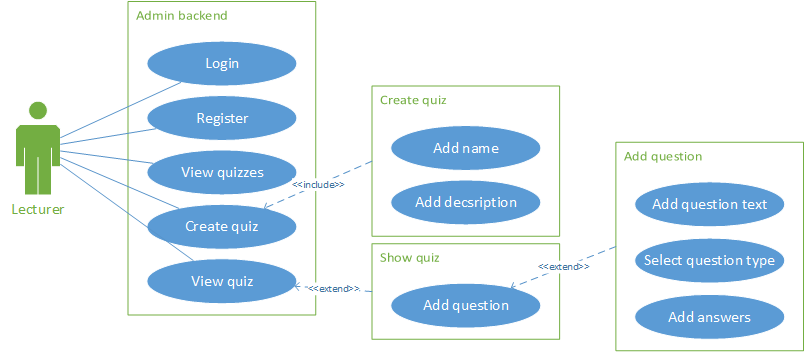
\includegraphics{Chapter2/Iter-2/iter-2-use-case-create}}
	\label{fig:quiz-create-use-case}
\end{figure}
\subsubsection{Implementation}
A create page was added for quizzes, this was linked to from the home page. This was mapped to /quizzes/create address. A simple form was added to this page with the name and description of the quiz. Questions would be added on an individual quiz page. The form sends the form as an HTTP POST request to the /quizzes page which then maps onto the 'Store' action in the Quiz Controller. This action is used for server side validation and saving the data to the database using an Eloquent function. This Eloquent function also returns the id of the new quiz. The user\_id is assigned to the quiz by simply getting the current user. Using this id, this Store function redirects to the newly created quiz.

On a quiz page, it displays the name and description and has a button to add any questions to the quiz. This button links to the questions/create page that functions in the same way as the quiz creation, albeit with the relevant fields in the form. The questions are assigned to the quiz by passing the quiz id to the question creation page in a GET variables via the url. This allows the question to be assigned to the quiz during its creation in the database and to be redirected back to the quiz page.

For validation there are two parts, one on the HTML form and the other handles server side. The HTML validation (client side) uses simple HTML 5 validation like the "required" attribute in the form inputs. Further frontend validation could be added utilising JavaScript but the HTML solution was far easier to implement, being the addition of one word and not several lines of code that have to be built and added to the correct pages. The server side complements this as client side validation can be circumnavigated by determined users.

The server side validation in Laravel is well supported and made as easy as possible to implement. The Store function used to save data from the POST request simply calls \textit{\$this-\textgreater validate()} on the request data. Inside this validation function, various rules can be imposed on individual pieces of the request data such as simply requiring that is is filled or that it has to have a minimum length\cite{laravel-validation}.

Something that Laravel enforces is the use of CSRF tokens to prevent cross site request forgery attacks on the site. A token is generated for the project during its creation, and this token must be placed in a hidden field within every form so that it can verify that the authenticated user is the one actually making the requests to the application\cite{laravel-csrf}.
\subsubsection{Testing}
A problem encountered in this set of tests is the speed of testing. Running six tests takes about a minute. The reason for this is that the tests use DatabaseMigrations rather than DatabaseTransactions, meaning that the database is migrated for every test. Using transactions would reduce the time taken by only doing a migration at the start and then using a transaction for each test. Alternatively having a pre migrated test database on which you run transactions would work too, but this would mean any time you change your database, you would have to remember to migrate the test database. TODO: describe transactions vs migrations

After attempting to use the transactions it appears as though they are not usable within Dusk. This is because Dusk is running in another process and migrations is the only choice\cite{dusk-transactions}. 
\newpage

\subsection{Story: They can edit an existing quiz they own}
\subsubsection{Analysis - breakdown of tasks}
\begin{itemize}
	\item There is an edit button on quizzes that links to quiz/edit
	\item You can edit the name of the quiz
	\item You can remove questions
	\item You can add questions
	\item You can edit the content of a question
	\item You can delete a quiz and its associated questions
\end{itemize}
\subsubsection{Design}
There was not much design for this stage as it only really adds an edit page which should look the same as the create pages in the above story except that the input fields are pre-filled with data that is being editing. Additionally a delete button should be added for quizzes and questions. (TODO: more design here) Figure \ref{fig:quiz-edit-use-case}
\begin{figure}
	\caption{Use case diagram for the admin backend with edit quiz functionality}
	\centerline{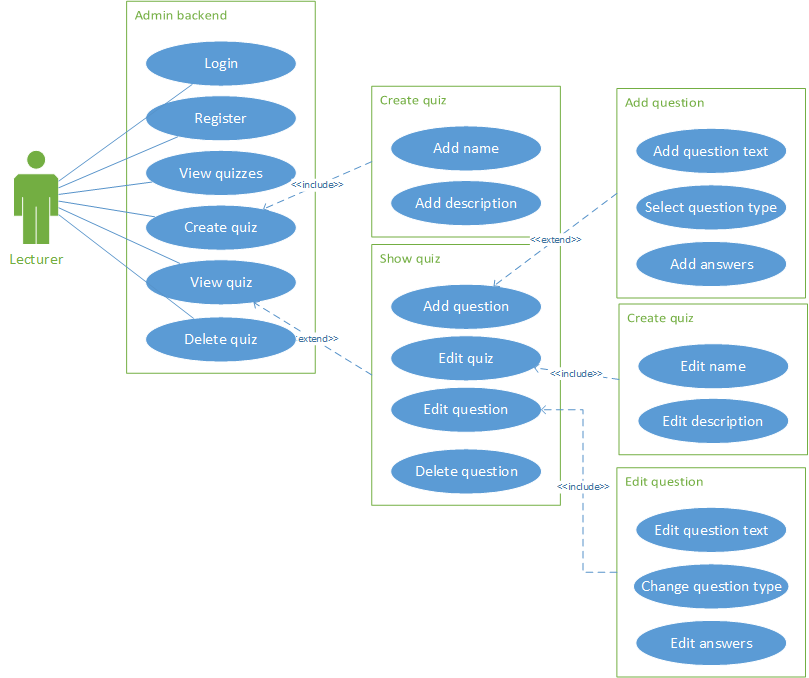
\includegraphics{Chapter2/Iter-2/iter-2-use-case-edit}}
	\label{fig:quiz-edit-use-case}
\end{figure}
\subsubsection{Implementation}
Pre filling the edit page was done by getting the record in the database by the id and just setting the default values of the input fields. The main difference to the creation stage was that the form had to use the HTTP PATCH method rather than POST. This PATCH method is automatically routed to the update function in the controller\cite{laravel-resource-controller}. Within this function, server side validation is performed and and Eloquent called to update the row in the database. It then redirects back to the quiz page for editing either a question or quiz.

Delete buttons were added to the quizzes and questions, these were not a simple \textless a \textgreater tag that linked to a delete page like the create and edit pages. This had to be a small form that sent an HTTP DELETE request along with an id to the /quizzes or /questions page. This was mapped to the destroy functions in the respective controllers which simply called an Eloquent function that removed the record. Due to the way the database is designed when a quiz or question is deleted, the linking row inside the quiz\_question table must also be deleted. 

Another thing that had to be changed was to make the foreign key reference columns in the quizzes and questions table cascade delete on deletion of the record. This meant that they would delete the rows in the quiz\_question table that referenced the row being deleted. For a quiz deletion, this had to go further and also find the questions associated with the quiz and delete all of those, which used a simple Eloquent function to find them using the quiz\_question table before the rows in that table were deleted and then delete the questions using those ids. 
\subsubsection{Testing}
Some simple tests written for editing and deleting quizzes and questions, no issues encountered.
\newpage

\subsection{Non-story work}
\subsubsection{Seeding}
Some more data needed to be seeded for this subsection of work, the question data. This involved creating some new Model Factories and using them in the seeders correctly. One issue was trying to create many questions for individual quizzes, but this was overcome using some very basic looping and calling the model factories in the right places.
\subsubsection{Quiz description}
It was decided that quizzes should probably have descriptions attached to them, in case the lecturer needs reminding of what it is in 6 months time. This involved creating a new migration and simply adding a column to the table.
\subsubsection{Travis setup}
Travis is a CI tool that can be used to run tests automatically on git pushes. Setting it up involved doing some spike work with another git project. It is really easy to set up, needing you to simply add a travis.yml file which specifies what Travis will do after a push. The project also has to be added from Github which is simple.
\newpage
